\chapter{\TLA}
\label{cap2}

\TLA é uma linguagem de especificação de software, criada por Leslie Lamport \cite{tlahistory} voltada à modelagem de sistemas concorrentes. Ela se propõe a oferecer uma maneira mais simples de escrever um algoritmo, ao utilizar um nível de abstração acima do que há ao escrever código em uma linguagem de programação. Assim, ao programar, não é necessário atentar-se a detalhes de implementação, permitindo o foco no comportamento do algoritmo - e não das suas dependências.

As especificações são descritas em fórmulas lógicas, com pequenas adaptações de sintaxe. Para facilitar a curva de aprendizado para engenheiros, foi criada a linguagem PlusCal \cite{pluscal}, com uma sintaxe semelhante a linguagens de programação imperativas, e que traduz seus programas para \TLAA. A linguagem PlusCal não permite especificar sistemas tão complexos quanto os que podem ser escritos diretamente em \TLAA, mas, devido à tradução para a linguagem original, aproveita completamente as capacidades dela de verificação de propriedades.

O método de especificação é baseado em máquinas de estados \cite{tlahistory} e, sendo assim, a descrição de um modelo é composta por uma condição inicial, que determina os possíveis estados iniciais, e por uma relação de transições, que determina os possíveis estados que podem suceder cada estado em uma execução. Dessa forma, o conjunto de comportamentos especificado é composto por todos os comportamentos cujo estado inicial satisfaz a condição inicial e todas as transições fazem parte da relação.

Lamport destaca \cite{hyperbook} que as especificações deveriam ser sobre modelos de uma abstração do sistema, e não algo retirado do próprio sistema. Semelhante à planta de um edifício, a especificação pode ser consultada para obter informações sobre o edifício (ou programa) de forma mais conveniente, além de ser capaz de facilitar uma série de verificações e perceber problemas enquanto a mudança ainda não é inviavelmente custosa.

Sendo assim, uma especificação em \TLA pode ser sobre comportamentos do ambiente no qual o programa funciona - como ao especificar um sistema e verificar possíveis comportamentos indesejáveis, entendendo aonde o programa deve atuar - des\-crevendo as operações existentes daquele sistema. Contudo, não limitada à definição de um sistema, uma especificação pode incluir comportamentos do programa em si, compostas por operações existentes do sistema e novas operações definidas pelo programa. Em seu livro \cite{specifying-systems}, Lamport define um sistema de memória linear e, então, propõe uma implementação de um programa de escrita através de \textit{cache} que atua sobre um sistema de memória linear. Assim, ele verifica que a especificação da implementação dele satisfaz a especificação do sistema e prova a implementação. Nos exemplos deste capítulo, serão explicadas especificações de sistemas e de implementações.

\section{Lógica Temporal das Ações}
\label{sec:tla}

\TLA combina a lógica TLA, proposta por Lamport em \cite{tlaformalization}, com teoria dos conjuntos - mais especificamente, a teoria de conjuntos de Zermelo-Fraenkel (ZFC), como detalhado em \cite{merzlogic}.

Lamport sumariza em \cite{proofsystem} o uso de TLA em \TLAA. TLA é uma lógica temporal linear. Em \TLAA, as variáveis rígidas do TLA são chamadas constantes, enquanto as flexíveis são chamadas variáveis. As constantes são declaradas com a palavra-chave \CONSTANTS e tem o mesmo valor para todos os estados de um comportamento - podendo diferir entre comportamentos. Já variáveis são declaradas com a palavra-chave \VARIABLES\ e podem ter valores diferentes em cada estado de um comportamento.

Os operadores são classificados em constantes e não constantes. Os constantes são aqueles que podem ser escritos em lógica clássica de primeira ordem. Os não constantes dependem de mais fatores, tal como o operador \textit{primed} ('), que depende do valor de uma variável em um estado diferente do atual. As definições em \TLA podem ser categorizadas em tipos de expressão. São denominadas fórmulas todas as expressões com valoração booleana.
\begin{itemize}
  \item \textbf{Expressões constantes} são expressões com apenas constantes declaradas e o\-pe\-ra\-do\-res constantes. Pela definição de operador constante, o valor de uma expressão constante depende apenas do valor das constantes contidas nela.
  \item \textbf{Expressões de estado} contém expressões constantes e variáveis declaradas. O valor de uma expressão de estado depende do estado, já que os valores das variáveis são definidos em um estado. Quando não são fórmulas, ou seja, sua valoração não é booleana, são chamadas também de funções de estado.
  \item \textbf{Expressões de ação} contém expressões de estado e operadores não constantes. O seu valor depende de um passo - um par de estados. Esse tipo de definição sobre ações dá o nome \textit{actions} a TLA, e pode ser chamado simplesmente de ação.
  \item \textbf{Expressões temporais} são permitidas apenas com valoração
    booleana em \TLAA, sendo assim, chamadas sempre de fórmulas temporais. Elas
    contém expressões de ação e operadores $\square$ e $\Diamond$ da lógica
    temporal (definidos posteriormente neste capítulo). O valor de uma fórmula
    temporal depende de uma sequência de passos, a que dá-se a denominação de comportamento.
\end{itemize}

Com essa estrutura, define-se a sintaxe na Figura \ref{fig:sintaxe-tla}. A hierarquia permite que toda a complexidade das definições em uma especificação esteja nas fórmulas de ações, e os operadores temporais sejam usados somente no momento de verificar propriedades de segurança, vivacidade e razoabilidade (\textit{fairness}).

\begin{figure}[h]
  \centering
  \fbox{$\begin{array}{l} \begin{array}{lrll}
    \text{Constantes} & c & ~~~~
    \text{Variáveis} & v \\
    \text{Estados} & s, t & ~~~~
    \text{Funções de estado} & f, g \\
    \text{Conjuntos} & S \\
    \end{array} \\ \\
    \begin{array}{lrcl}
  \text{Ação} & \FANCYA & ::= & c \,\mid\, v \,\mid\, v' \,\mid\, \neg \FANCYA \,\mid\, \FANCYA \land \FANCYA \smallskip\\
  \text{Predicado} & P, Q & ::= & c \,\mid\, v \,\mid\, \neg P \,\mid\, P \land P \,\mid\, \ENABLED \FANCYA\smallskip\\
  \text{Fórmula Simples} & F & ::= & P \,\mid\, [\FANCYA]_f  \mid\, \langle\FANCYA\rangle_f \,\mid\,  \neg F \,\mid\,  F \land F  \,\mid\, \square F \smallskip\\
  \text{Fórmula Geral} & G & ::= & F \,\mid\, \EE x : G  \,\mid\, \neg G \,\mid\,  G \land G \mid\, G \implies G \smallskip\\
  \end{array} \end{array}$}
  \caption{Sintaxe da linguagem de TLA}
\label{fig:sintaxe-tla}
\end{figure}

Uma fórmula temporal em TLA é verdadeira ou falsa em um comportamento, que é definido por uma sequência infinita de estados. Uma fórmula é dita válida se e somente se ela é verdadeira para todos os comportamentos. Assim, a especificação de um sistema é dada por uma fórmula geral $G$ e representa um sistema cujo conjunto de comportamentos permitidos é igual ao conjunto de comportamentos que satisfazem $G$.

Implementação é representada através de implicação. Uma especificação dada pela fórmula $G_0$ implementa outra especificação dada por $G_1$ se e somente se qualquer sistema cujo conjunto de comportamentos satisfaz $G_0$ também satisfaz $G_1$, ou seja, a fórmula $G_0 \implies G_1$ é válida.

Em \cite{tlaformalization}, são definidas também notações auxiliares. A lista abaixo apresenta a definição e atribui um possível significado a possíveis operadores para fórmulas temporais:
\begin{itemize}
  \item $\square F$ ($F$ é sempre verdadeiro) para uma fórmula temporal $F$ é satisfeito por um comportamento se e somente se $F$ é verdadeiro para todos os sufixos (primeiro estado em um passo) do comportamento.

  \item $\Diamond F$ (Eventualmente $F$) é definido como $\neg \square \neg F$. Ou
    seja, não é sempre que $F$ será falso.

  \item $F_0 \leadsto F_1$ (Em qualquer momento em que $F_0$ for verdadeiro, $F_1$ eventualmente será) é definido como $\square(F_0 \implies \Diamond F_1)$

  % \item $F \stackrel{+}\rightarrow G$ para fórmulas temporais $F$ e $G$ é verdadeiro para um comportamento se e somente se $G$ é verdadeiro, pelo menos, enquanto $F$ é.

  \item \EE $x : F$, para uma variável $x$ e uma fórmula temporal $F$, é satisfeito por comportamento se e somente se existem alguns valores a serem atribuídos a $x$ que produzem um comportamento que satisfaz $F$. Esse operador é uma especialização do quantificador existencial comum $\E$ porque ele asserte a existência de uma sequência infinita de valores para $x$, e não um único valor.

\end{itemize}

Para ações, são definidos ainda outros operadores:

\begin{itemize}
  \item $f'$ (f \textit{primed}) para uma função de estado $f$ é o valor de $f$
    no final de um passo. Em outras palavras, para um passo composto por uma
    dupla de estados $<s, t>$, $f'$ é o valor de $f$ para $t$. De forma semelhante, $P'$ para um predicado $P$ é o valor de $P$ para o estado final de um passo. Assim, na avaliação da valoração de uma ação para um passo, predicados e variáveis sem o operador \textit{primed} se referem aos seus respectivos valores no primeiro estado do passo, e sempre que forem marcados com o operador, fazem referência aos valores no segundo estado do passo.

  \item A fórmula $[\FANCYA]_f$ para uma ação $\FANCYA$ e uma função de estado
    $f$ é satisfeita por um  passo que satisfaz \FANCYA ou mantém o valor de $f$ - ou seja, $\FANCYA \lor (f = f')$.

  \item A fórmula $\langle\FANCYA\rangle_f$ para uma ação $\FANCYA$ e uma função
    de estado $f$ é satisfeita por um passo que satisfaz \FANCYA e altera o valor de $f$ - ou seja, $\FANCYA \land (f \neq f')$.

  \item \ENABLED \FANCYA (\FANCYA é ativável) para uma ação \FANCYA é um predicado cujo valor é verdadeiro para um estado $s$ se e somente se é possível fazer um passo \FANCYA partindo de $s$. Isto é, existe um estado $t$ tal que o passo formado pelo par $s$ e $t$ satisfaz \FANCYA.

  \item \UNCHANGED $f$ ($f$ não é modificado) para uma fórmula de estado $f$ em um passo (par de estados) é definido como $f' = f$  (o valor de $f$ no estado atual é igual ao valor de $f$ no próximo estado).

\end{itemize}

TLA conta com muitos operadores constantes, trazidos da matemática, da lógica, da teoria de conjuntos e de linguagens de programação. Abaixo, são apresentados os considerados menos triviais, sendo que a lista completa é definida em \cite{specifying-systems}.

\begin{itemize}

  \item \CHOOSE $x \in S : P$ (escolha algum $x$ pertencente ao conjunto $S$ que satisfaça $P$) para uma variável $x$ e um predicado $P$ resulta em algum valor de $x$ que satisfaz $P$ se \EE $x : P$ for verdadeiro. Sobre \CHOOSE, é possível afirmar que se \EE $x : P$ então $P(\CHOOSE x \in S : P)$ é verdadeiro, e que para todo predicado $Q$ tal que $Q \equiv P$, é verdade que $(\CHOOSE x \in S : P) = (\CHOOSE x \in S : Q)$.

  \item $f \EXCEPT ![v] = e$ para uma função $f$, um elemento de seu domínio $v$ e uma expressão $e$ resulta em uma cópia de $f$ exceto pelo valor $f[v]$ que é igual a $e$.

  \item $[h_1 \mapsto e_1, \dots, h_n \mapsto e_n]$ é uma estrutura do tipo registro (\textit{record}) onde $h_i$ são campos e $e_i$ são expressões constantes para os valores de $h_i$. O valor de um campo $h$ qualquer em um registro $r$ pode ser obtido por $r.h$, e o operador $r \EXCEPT !h = e$ funciona de forma semelhante ao definido no item anterior, retornando uma cópia de $r$ exceto pelo valor de $r.h$, que é $e$.

  % \item \ASSUME $c$ (assuma $c$) para uma fórmula constante $c$ define $c$ como verdadeiro. Esse operador não tem nenhum efeito nas definições de uma especificação, apenas pode facilitar a verificação de teoremas.
\end{itemize}

Finalmente, os operadores lógicos $\land$ e $\lor$ podem ser prefixados às expressões, sendo

\begin{center}
  $\begin{array}{lll}
\begin{array}{ll}
  \land\ e_1\\
  \vdots ~~~~ & \equiv ~~~~ e_1 \land \dots \land e_n\\
  \land\ e_n
\end{array} &
~~~~ e ~~~~ &
\begin{array}{ll}
  \lor\ e_1\\
  \vdots ~~~~ & \equiv ~~~~ e_1 \lor \dots \lor e_n\\
  \lor\ e_n
\end{array}
\end{array}$
\end{center}

\subsection{Passos balbuciantes}

Os passos balbuciantes (\textit{stuttering steps}) são parte importante das especificações em TLA. Eles permitem que o estado - formado pelos valores das variáveis da especificação - se mantenha igual durante um passo.

Supondo que as variáveis da especificação estejam declaradas como
\[vars = \langle var_1, var_2, \dots, var_n\rangle\]

Então é possível usar o operador $\square [\FANCYA]_f$ definido, com $f = vars$, no seguinte teorema sobre uma especificação $Spec$

\[\THEOREM Spec \implies \square [\FANCYA]_{vars}\]

\noindent o que, se verificado, garante que cada passo de um comportamento satisfeito por $Spec$ satisfaz a ação \FANCYA ou é um passo balbuciante e mantém os valores das variáveis em $vars$. Isso é importante porque possibilita que nem todos os passos do sistema sejam especificados - seria muito complexo definir tudo o que pode ocorrer durante sua execução. Assim, definem-se apenas os passos relevantes para o sistema, e todos os outros passos - aqueles que não alteram as variáveis definidas - são permitidos. Um comportamento que passa a ter infinitos passos balbuciantes pode significar uma execução do sistema que finalizou. Com a definição de passos balbuciantes, é possível definir as propriedades apresentadas na Seção \ref{propriedades}.

\section{Propriedades}
\label{propriedades}

Sobre uma especificação definida, \TLA permite a verificação de algumas propriedades de segurança e vivacidade. Essas propriedades são descritas em forma de teoremas na especificação apenas com o intuito de documentar sua verificação, porém devem ser inseridas manualmente no modelo TLC para serem, de fato, checadas.

Propriedades são fórmulas temporais sobre ações definidas na especificação. Uma propriedade é satisfeita se a fórmula temporal que a define é válida.

\subsection{Propriedades de Segurança}

Propriedades de segurança definem o que o sistema pode fazer. Quando uma propriedade de segurança é violada, ela é violada em um instante específico de um comportamento. Esse tipo de propriedade é definido em \TLA como uma invariante.

Uma invariante é um predicado $P$ que é verdadeiro em todos os passos de todos os comportamentos permitidos por uma especificação $Spec$, e pode ser verificada com a prova do teorema

\[\THEOREM Spec \implies \square P\]

\subsection{Propriedades de Vivacidade}

Propriedades de vivacidade definem o que o sistema deve fazer. Quando uma propriedade de vivacidade é violada, ela é violada em um comportamento. Em \cite{specifying-systems}, é apresentada uma especificação para um relógio. O ponteiro de um relógio deve, eventualmente, mexer. Esse é um tipo de propriedade que pode ser descrita com uma propriedade de vivacidade, tal qual a razoabilidade fraca (\textit{weak fairness}).

A razoabilidade fraca para uma fórmula de estado $f$ e uma ação \FANCYA é escrita como $WF_f (\FANCYA)$. Ela é satisfeita por um comportamento se e somente se \FANCYA $\land\ (f' \neq f)$ é infinitamente não ativável (\textsc{enabled}) ou infinitos passos \FANCYA $\land\ (f' \neq f)$ ocorrem. Sendo assim, essa propriedade garante que \FANCYA não possa permanecer continuamente ativável para sempre sem que um passo \FANCYA ocorra. Essa condição pode ser escrita de forma equivalente como

\[\square (\ENABLED \FANCYA \implies \Diamond\langle\FANCYA\rangle_f)\]

A conjunção com $(f' \neq f)$, expressada com a notação $\langle\FANCYA\rangle_f$, se deve ao fato de não ser desejável exigir que passos balbuciantes eventualmente ocorram. \FANCYA $\land\ (f' \neq f)$ pode ser lido como "todos os passos não balbuciantes que satisfazem \FANCYA".

A razoabilidade fraca recebe a denominação "fraca" porque exige que uma ação permaneça continuamente ativável para garantir a ocorrência de um passo satisfazendo-a. Se um comportamento repetidamente tornar a ação ativável e em seguida não ativável, a razoabilidade fraca não garante nada sobre a ocorrência da ação neste comportamento. Para tal, é necessário garantir a propriedade de razoabilidade forte (\textit{strong fairness}).

A razoabilidade forte para uma fórmula de estado $f$ e uma ação \FANCYA é escrita como $SF_f (\FANCYA)$. Ela é satisfeita por um comportamento se e somente se \FANCYA $\land (f' \neq f)$ ocorre finitas vezes ou infinitos passos \FANCYA $\land (f' \neq f)$ ocorrem. Essa propriedade garante que \FANCYA não possa ser repetidamente ativável para sempre sem que um passo \FANCYA ocorra. Uma forma equivalente de representar essa condição é

\[\square \Diamond \ENABLED \FANCYA \implies \square \Diamond\langle\FANCYA\rangle_f\]

que pode ser lida como "se sempre \FANCYA for eventualmente ativável, então sempre um passo $\langle\FANCYA\rangle_f$ deve eventualmente ocorrer".

\section{Exemplo 1 - Jarros de Água}
\label{exemplo1}

Para exemplificar uma especificação de um sistema, é possível definir um
problema combinatório simples como o dos jarros de água, como Lamport faz em \cite{video-protocol}. Nesse problema, são fornecidos dois jarros inicialmente vazios, um com capacidade de 3 litros e outro com capacidade de 5 litros, assim como uma fonte inesgotável de água. Sendo assim, é possível despejar a água dos jarros no chão, transferir a água de um jarro ao outro ou encher um jarro com a fonte de água.

O objetivo do problema é ter exatamente 4 litros de água em um dos jarros. Isso é, dada uma máquina de estados, é necessário encontrar uma sequência de transições que leva a algum estado onde o jarro maior tem exatamente 4 litros de água. No entanto, para esse exemplo, deseja-se apenas especificar os comportamentos do sistema em si, e não de um possível programa que buscaria atingir esse objetivo. Uma possível especificação em \TLA para esse sistema se encontra na Figura \ref{fig:ex1tla}.

\begin{figure}
  \centering
  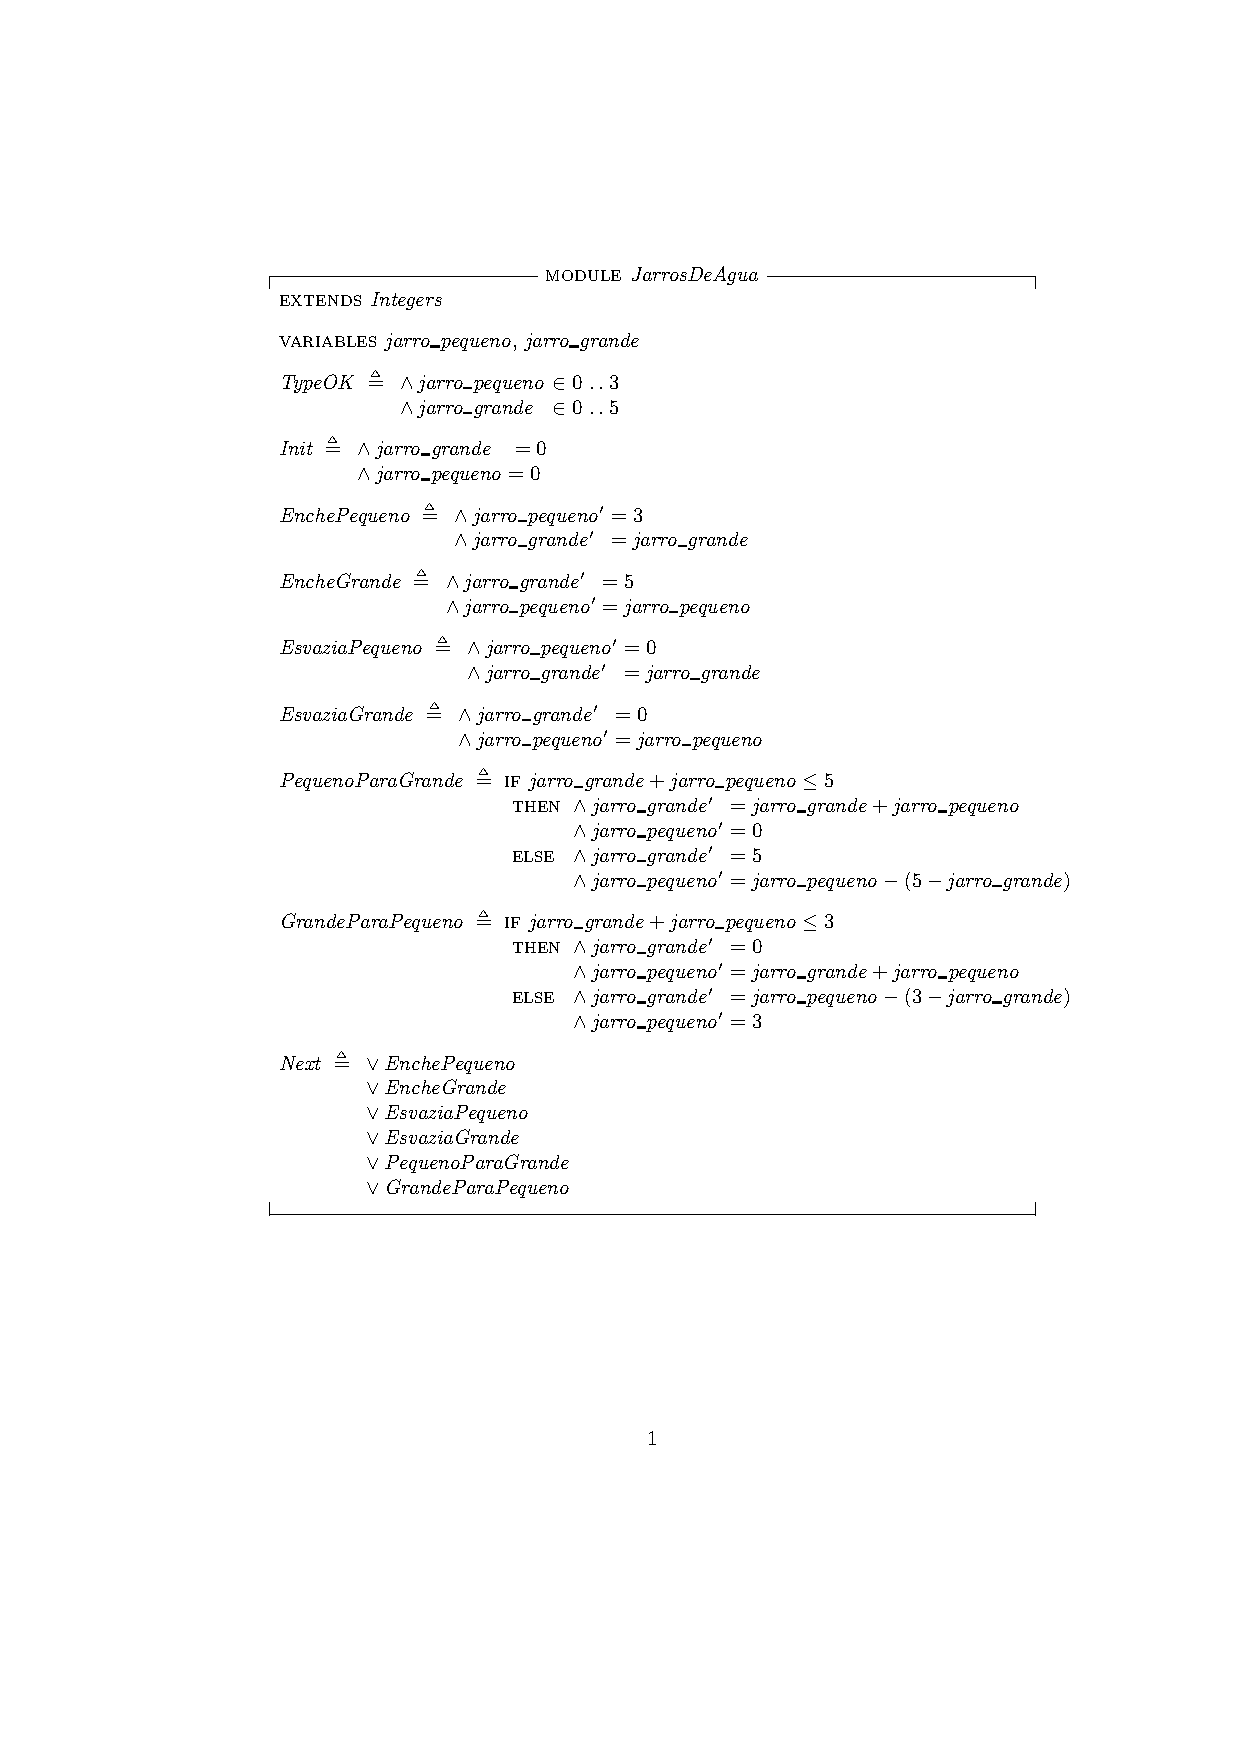
\includegraphics[width=\textwidth]{fig/JarrosDeAgua.png}
  \caption{Especificação do problema dos Jarros de Água}
  \label{fig:ex1tla}
\end{figure}

Entendendo essa especificação no modelo de máquina de estado, é possível observar que as variáveis (\VARIABLES) são um conjunto de valores que variam nos estados, de forma que o conjunto com todas as combinações dos valores possíveis para cada uma das variáveis forma o conjunto de estados da máquina. Um estado desse sistema seria $jarro\_pequeno = 0, jarro\_grande = 1$. Na definição $Init$, é especificada uma fórmula que determina estados iniciais válidos - o que, nesse caso, é apenas o estado onde todas as variáveis do sistema tem valor 0.

As seis definições seguintes representam as transições através de ações. Em cada uma delas, as variáveis com o operador \textit{primed} (') representam os valores no estado seguinte, e sempre precisam ser definidas. Na transição $EnchePequeno$, o valor de $jarro\_grande$ se mantém o mesmo entre os estados atual e seguinte, mas é necessário explicitar isso com $jarro\_grande' = jarro\_grande$. Essa necessidade vem da aproximação da sintaxe de \TLA com a matemática, onde não existe efeito colateral e, portanto, o valor da variável $jarro\_grande$ não propaga de um estado para outro.

É possível, sintaticamente, utilizar a informação das variáveis do estado a\-tu\-al para definir o estado seguinte - não é necessário definir exaustivamente transições para todas as combinações de variáveis. Dessa forma, as ações definidas representam transições para vários estados do sistema. Cada transição da especificação do problema dos jarros pode ser aplicada em qualquer um dos estados, isto é: $(jarro\_pequeno = 0,\ jarro\_grande = 0), (jarro\_pequeno = 0,\ jarro\_grande = 1), \dots$.

No sentido de aproveitar informações do estado atual, é possível utilizar condicionais, como nas ações $PequenoParaGrande$ e $GrandeParaPequeno$. Com isso, é fácil definir transições diferentes para conjuntos de estados com propriedades diferentes. Na definição de $PequenoParaGrande$, os estados que atualmente possuem 5 litros ou menos de água nos jarros em total recebem uma transição para um estado onde o jarro pequeno está vazio. Já os estados que possuem mais de 5 litros de água recebem uma transição para um estado onde o jarro grande está cheio.

Ao fim dessa especificação, em $Next$, é definida a \textit{next state function} (função de próximo estado), na qual são declaradas as fórmulas transicionais do sistema, incluindo qualquer composição dessas fórmulas que possa levar um estado a outro. No caso do problema dos jarros, apenas é definido que qualquer transição pode ser utilizada para obter um novo estado.

As definições $Init$ e $Next$ são buscadas pelo \textit{model checker} TLC na construção da máquina de estados. É possível renomear essas definições, mas é preciso informar ao TLC os novos nomes para o estado inicial e a \textit{next state function}. A especificação - chamada $Spec$ - é descrita a partir dessas definições com a fórmula temporal

\[Spec \defeq Init \land \square [Next]_{vars}\]

Onde $vars$ é uma tupla contendo todas as variáveis declaradas. Com essa especificação, o sistema está definido. As operações permitidas e as variáveis relevantes foram descritas e, a partir do estado inicial, cada passo do sistema pode ser executado a partir de uma das seis diferentes ações ou de passos balbuciantes sobre $vars$. Essas informações são suficientes para o TLC fazer verificações sobre o sistema, é apenas necessário definir tais verificações.

A definição $TypeOK$ na especificação apresentada pode ser utilizada para verificar os tipos desse sistema. Ela define que a variável $jarro\_pequeno$ é sempre um inteiro entre 0 e 3, e a variável $jarro\_grande$ é sempre um inteiro entre 0 e 5. Ou seja, $TypeOK$ será verdadeiro se e somente se os valores das variáveis estiverem de acordo com essas restrições. Isso não é uma verificação em si, e sim uma definição. Para que essa definição seja verificada em todos os estados alcançáveis pelo sistema, é necessário adicioná-la como uma invariante do modelo. Como uma invariante, o valor dela deve ser verdadeiro para todos os estados da execução. Assim, ao definir essa invariante, todos os estados devem fazer $TypeOK$ verdadeiro, ou o TLC retornará um erro. $TypeOk$ pode ser definido como uma invariante através do teorema:

\[\THEOREM Spec \implies \square (TypeOK)\]

Outra propriedade interessante de ser verificada para esse problema antes da
implementação de um programa para resolvê-lo é a possibilidade de resolução,
isto é, se é possível alcançar um estado onde onde o jarro maior contém 4 litros
de água. Para isso, define-se uma invariante para o predicado $jarro\_grande\
\backslash= 4$ (onde $\backslash=$ é operador da diferença), que não será satisfeita. Como esse predicado é verdadeiro para o estado inicial, o fato de ele não ser satisfeito significa que, em algum momento da execução, o predicado foi falso, ou seja, $jarro\_grande = 4$. Adicionando essa invariante, um possível teorema seria:

\[\THEOREM Spec \implies \square (TypeOK \land jarro\_grande\ \backslash= 4)\]

O TLC, ao encontrar uma execução que insatisfaz a invariante, traz a sequência de transições que levam ao estado onde o predicado é falso, o que, no caso do simples problema dos jarros, é a solução buscada.

Esse exemplo é apresentado com o intuito de demonstrar a estrutura da especificação de um sistema e o funcionamento das invariantes. A seguir, é proposto um exemplo com a especificação de um sistema real que pode ser implementado por especificações de programas para verificar que as propriedades definidas são mantidas. % e de um protocolo implementado sobre ele.

\section{Exemplo 2 - Transações em Bancos de Dados}
\label{exemplo2}

Já tratando de um contexto de um problema real de sistemas concorrentes,
define-se uma especificação para o problema da consistência das transações em
bancos de dados \cite{video-protocol}. Esse é um problema clássico onde, dado um conjunto de gerenciadores de recursos fazendo operações sobre um mesmo banco, um gerenciador só pode efetivar (fazer a ação \textit{commit}) se todos os outros gerenciadores estiverem preparados para efetivar; e se algum gerenciador quiser abortar, então todos devem abortar. Ou seja, em nenhum momento pode haver um gerenciador abortado e outro cometido.

\subsection{O sistema}

Na Figura \ref{fig:ex2tla}, encontra-se uma especificação para um sistema de transações consistente. Ela não apresenta uma proposta de solução para o problema, e sim traz uma descrição formal do que significa ser consistente quando se trata de transações. Uma especificação de uma solução para o problema deve implementar essa especificação.

\begin{figure}[h]
  \centering
  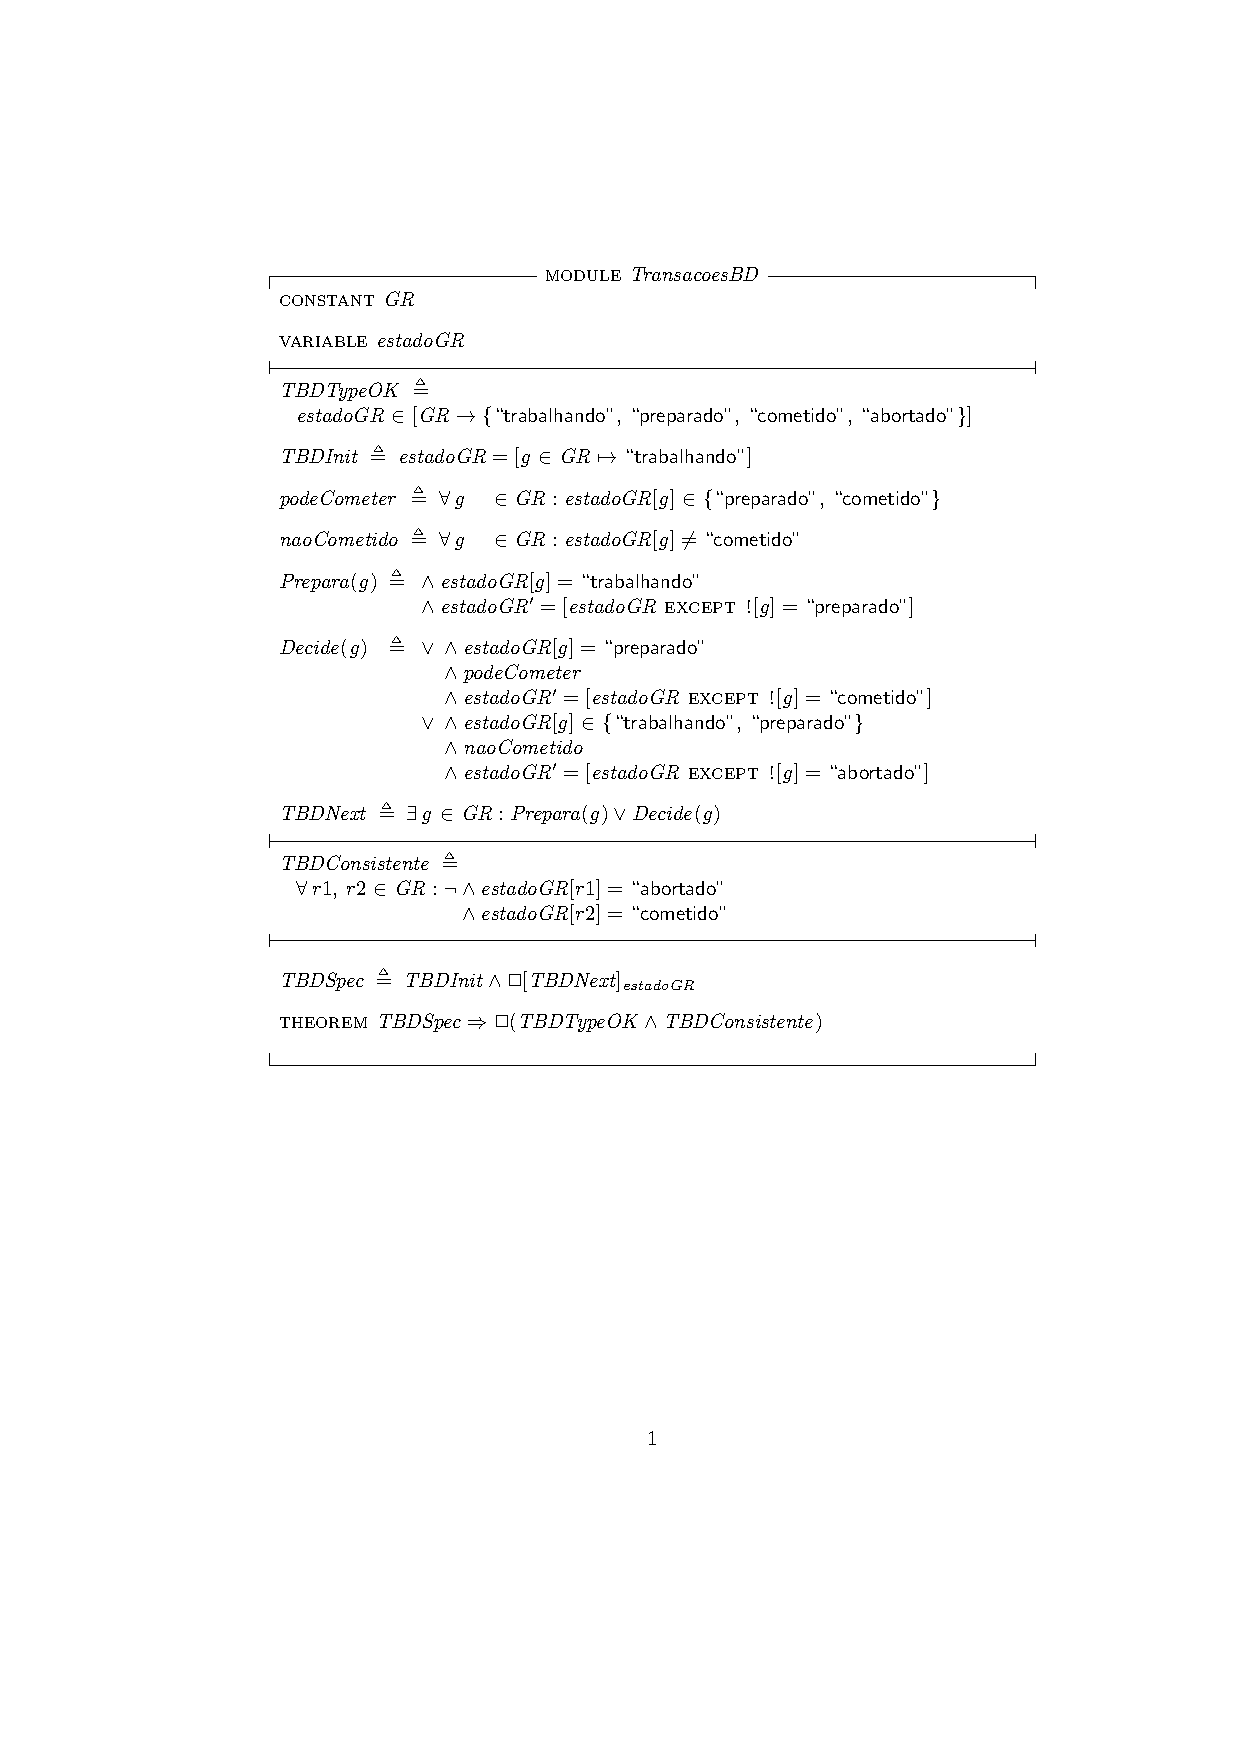
\includegraphics[width=\textwidth]{fig/TransacoesBD.png}
  \caption{Especificação de um sistema de transações em bancos de dados}
\label{fig:ex2tla}
\end{figure}

Um gerenciador de recursos pode estar em quatro estados diferentes, como definido em $TBDTypeOK$. Do estado \trabalhando, ele pode ir para o estado \preparado, no sentido de que ele está pronto para efetivar; ou então abortar, indo para o estado \abortado. Se todos os gerenciadores estão no estado \preparado, então qualquer um deles pode efetivar, indo para o estado \cometido; ou então abortar, indo para o estado \abortado. Contudo, se exite algum gerenciador no estado \cometido, então nenhum outro gerenciador pode abortar.

A possibilidade de um gerenciador $g$ ir do estado \trabalhando\ ao \preparado\ é representada pela ação $Prepara(g)$ onde, se o estado de $g$ é \trabalhando, então o valor da variável $estadoGR$ no novo estado é igual ao seu valor no estado atual, exceto pelo valor de $estadoGR[g]$, que passa a ser \preparado.

A decisão de um gerenciador de abortar ou efetivar é representada pela ação
$Decide(g)$. Nessa definição, as fórmulas $podeEfetivar$ e $naoEfetivado$ são
definidas separadamente para minimizar a complexidade cognitiva da especificação
- definí-las dentro de $Decide(g)$ seria semanticamente equivalente.
$podeEfetivar$ verifica se todos os estados estão preparados ou cometidos, ou seja, qualquer um pode efetivar. Se $podeEfetivar$ for verdadeiro, e $g$ ainda não cometeu, então $g$ comete - o estado dos gerenciadores passa a ser uma cópia do estado atual exceto por $estadoGR[g]$, que é \cometido. Outra decisão possível, separada da primeira por um operador de disjunção, é a de abortar. Para isso, verifica-se, com a fórmula $naoEfetivado$, se não há nenhum gerenciador cometido. Se $naoEfetivado$ for verdadeira, e $g$ ainda não tiver abortado, então o novo estado dos gerenciadores passa a ter $g$ como \abortado.

Com essas fórmulas, é possível definir a \textit{next state function} $TBDNext$, onde um passo do sistema é dado por um gerenciador de recursos no conjunto $GR$ que faz uma ação de preparar ou decidir. A fórmula temporal $TBDSpec$ consiste a especificação do sistema de transações bancárias e tem um formato semelhante à fórmula $Spec$ do exemplo anterior, na Seção \ref{exemplo1}.

Para verificar que o sistema especificado por $TBDSpec$ está de acordo com a restrição do problema - em nenhum momento pode haver um gerenciador abortado e outro cometido - define-se $TBDConsistente$ onde, para cada possível par de gerenciadores de recursos, não é o caso de o primeiro estar abortado e o segundo, cometido. Essa fórmula é uma afirmação sobre um valor da variável $estadoGR$, porém precisa ser verdadeira para todos os valores dessa variável em qualquer comportamento que satisfaça $TBDSpec$. Para isso, ela é definida como uma invariante através do teorema

\[\THEOREM TBDSpec \implies \square(TBDTypeOK \land TBDConsistente)\]

que permite verificar que, se um comportamento satisfaz $TBDSpec$ - isto é, seu
estado inicial satisfaz $TBDInit$ e seus passos satisfazem $TBDNext$ - então os
predicados $TBDTypeOK$ e $TBDConsistente$ são verdadeiros para todas as estados
- todos os valores atribuídos para as variáveis - neste comportamento. Sendo
satisfeito esse teorema, $TBDTypeOK$ e $TBDConsistente$ são ambos invariantes da especificação.

\subsection{O protocolo}
\label{sec:protocolo}

A partir da definição de ações válidas em um sistema de transações, é possível
especificar um protocolo que restringe as ações de forma a atender propriedades
desejadas. A estratégia de definir um protocolo com esse objetivo está presente
em diversos contextos, como ao abrir uma nova conta bancária. Ao especificar um
protocolo em \TLAA, é possível verificar as propriedades que ele busca atender e
garantir que está cumprindo seu propósito.

Para o sistema de transações em bancos de dados, Lamport define em
\cite{video-protocol} o protocolo de efetivação em duas fases. Esse protocolo
estabelece que os gerenciadores de recurso se comuniquem com um gerenciador de
transações (GT), avisando quando estão preparados para efetivar uma transação.
Quando todos os gerenciadores de recurso estão preparados ($GRsPreparados =
GR$), o gerenciador de transações envia uma mensagem a todos os gerenciadores de
recurso para que efetivem.

A Figura \ref{fig:ex3tlap1} apresenta a primeira
parte da especificação desse protocolo, onde são definidas as ações para o
gerenciador de transações. A ação $GTRecebePrepara$ acontece quando uma mensagem
``EstouPreparado'' é recebida e coloca o gerenciador de recurso $g$ que enviou a
mensagem no conjunto de gerenciadores preparados $GRsPreparados$. Quando todos
os gerenciadores estão preparados, a ação $GTEfetiva$ se torna ativável, podendo
enviar o comando ``Efetive'' para os gerenciadores.

Adicionalmente, o gerenciador de transações pode abortar espontaneamente. Essa
característica é definida por $GTAborta$, que pode ocorrer a qualquer momento em
que o gerenciador esteja ativo, isto é, $estadoGT = ``inicio"$.

\begin{figure}[hb]
  \centering
  \includegraphics[width=\textwidth]{fig/EfetivacaoEmDuasFases1.png}
  \caption{Especificação do protocolo de efetivação em duas fases - Parte 1}
\label{fig:ex3tlap1}
\end{figure}

\begin{figure}[ht]
  \centering
  \includegraphics[width=\textwidth]{fig/EfetivacaoEmDuasFases2.png}
 \caption{Especificação do protocolo de efetivação em duas fases - Parte 2}
\label{fig:ex3tlap2}
\end{figure}

A Parte 2 da especificação, na Figura \ref{fig:ex3tlap2}, contém as definições
de ações para os gerenciadores de recurso. Elas são semelhantes àquelas da
especificação do sistema de transações, na Figura \ref{fig:ex1tla}, exceto que
nessa especificação o $estadoGR$ só alterado se uma mensagem de abortar ou
efetivar for recebida, e não diretamente após o gerenciador escolher abortar ou efetivar.

$DFNext$ que qualquer ação para qualquer gerenciador de recurso pode acontecer a
qualquer momento, e $DFSpec$ obedece o mesmo formato das especificações
apresentadas até então. O teorema $\THEOREM DFSpec \implies \square DFTypeOK$
define o predicado sobre tipos como uma invariante, e com as declarações
\[\INSTANCE TransacoesBD\]
\[\THEOREM DFSpec \implies TBDSpec\]

as definições da especificação do sistema são importadas e, ao verificar que
$DFSpec \implies TBDSpec$, garante-se que as ações do protocolo respeitam as
propriedades exigidas por $TBDSpec$ - a especificação do sistema. Em outras
palavras, $DFSpec$ implementa $TBDSpec$.


\subsubsection{Troca de mensagens}

O conjunto $msgs$ dessa especificação contém todas as mensagens que em algum
momento foram enviadas, uma vez que em nenhum momento uma mensagem é retirada do
conjunto. Isso significa que uma mensagem pode ser recebida qualquer número de
vezes e, no contexto dessa especificação, isso não é um problema, já que a ação
executada ao receber mensagens pode ser feita uma ou infinitas vezes sem alterar
o resultado.

Apesar de modelar a troca de mensagens da maneira mais simples possível fazer todo o sentido para uma especificação, fazer uma implementação com esse tipo de estrutura não seria viável, já que as ações são executadas por processos e os recursos são finitos. O protocolo de efetivação em duas fases não é um algoritmo a ser implementado, e isso permite que extrapolações como essas sejam presentes em sua especificação. O protocolo não determina como fazer a troca de mensagens - isso não faz parte da sua responsabilidade - e uma implementação desse protocolo deve definir uma forma de fazê-lo que seja viável e que satisfaça o protocolo.

\subsubsection{Escolhas}

$DFNext$ define que qualquer ação para qualquer gerenciador de recurso é válida
como um próximo passo, ou seja, dado um passo de um estado $s$ para outro
estado $t$, qualquer ação satisfeita pela dupla $<s, t>$ pode ocorrer como
próximo passo.

A influência dos valores de $s$ e $t$ na satisfação de ações, contudo, pode
variar. Dado um momento onde o estado $s$ possui o valor de $msgs$ igual a
$\{[tipo \mapsto ``Efetive"]\}$, as ações $GRRecebeMsgAborte(g)$ não poderiam ser
satisfeitas para nenhum valor de $t$, já que há nelas o predicado $[tipo \mapsto
``Aborte"] \in msgs$. Se o estado também possuir o valor de
$estadoGR$ igual a ``preparado'' para todo gerenciador $g \in GR$, as ações
$GRPrepara(g)$ e $GREscolheAbortar(g)$ também não poderiam ser satisfeitas, já
que exigem um gerenciador no estado ``trabalhando''.

Em alguns casos, apenas olhando para o valor do estado atual, é possível filtrar
ações disjuntivas a ponto de apenas uma ação ser possivelmente satisfeita. Se
essa ação define o valor de todas as variáveis no próximo estado - através de
operadores \textit{primed} e $\UNCHANGED$ - então esses valores são os únicos
possíveis para as variáveis do próximo estado.

Em outros casos, encontrar apenas uma possível ação a partir do estado atual nunca será possível. As
ações $GRPrepara(g)$ e $GREscolheAbortar(g)$ para um mesmo gerenciador $g$, por
exemplo, tem um único predicado e ele é idêntico para ambas: $estadoGR[g] =
``trabalhando"$. Uma vez que essas ações exigem próximos estados diferentes pelo
valor de $estadoGR'$, sabe-se que a partir de um estado $s$ que satisfaça-as,
sempre haverá mais de um próximo estado possível que satisfaça a especificação.

Se a disjunção do conjunto de ações cujos predicados são satisfeitos pelo estado
atual $s$ é satisfeita por mais de um valor de próximo estado $t$, o estado
atual exige uma escolha. Para a lógica temporal e o TLC, essas situações representam uma ramificação
na árvore de estados.

Uma escolha no protocolo efetivação em duas fases, por exemplo, é a de um
gerenciador de recurso preparar ($GRPrepara(g)$) ou abortar ($GREscolheAbortar(g)$).
Escolhas não estão definidas pela especificação, e nesse caso poderia ser dada pelo
resultado de uma etapa da transação de um gerenciador de recursos, onde ele pode
escolher preparar (se o resultado foi sucesso) ou abortar (caso o resultado
tenha sido fracasso); ou então poderia ser dada por um fator aleatório; isso não
é relevante para o modelo especificado - qualquer escolha é válida.

